\documentclass[10pt,a4paper]{article}
\usepackage[utf8]{inputenc}
\usepackage[T1]{fontenc}
\usepackage{amssymb}
\usepackage{graphicx}
\usepackage{mathtools}
\usepackage{amsthm}
\usepackage{thmtools}
\begin{document}
Trig identities:
\\	$\frac{d}{dx}(\sin{x}) = \cos{x}$
\\	$\frac{d}{dx}(\cos{x}) = -\sin{x}$
\\	$\frac{d}{dx}(\tan{x}) = \sec^{2}{x}$
\\	$\frac{d}{dx}(\csc{x}) = \csc{x}\cot{x}$
\\	$\frac{d}{dx}(\sec{x})= \sec{x}\tan{x}$
\\	$\frac{d}{dx}(\cot{x}) = -\csc^{2}{x}$
\\	$\frac{d}{dx}(\sin^{-1}{x}) = \frac{1}{\sqrt{1-x^{2}}}$
\\	$\frac{d}{dx}(\cos^{-1}{x}) = -\frac{1}{\sqrt{1-x^{2}}}$
\\	$\frac{d}{dx}(\tan^{-1}{x}) = \frac{1}{1+x^{2}}$
\\ $\frac{d}{dx}(\cot^{-1}{x}) = -\frac{1}{1+x^{2}}$
\\ $\frac{d}{dx}(\sec^{-1}{x}) = \frac{1}{x\sqrt{x^{2}-1}}$
\\ $\frac{d}{dx}(\csc^{-1}{x}) = -\frac{1}{x\sqrt{x^{2}-1}}$	
\\Anti derivatives to know:	
\\	$cf(x) \rightarrow cF(x)$
\\	$f(x) + g(x) \rightarrow F(x) + G(x)$
\\	$x^{n}(n \neq -1) \rightarrow \frac{x^{n+1}}{n+1}$
\\	$\frac{1}{x} \rightarrow \ln{|x|}$
\\	$e^{x} \rightarrow e^{x}$
\\	$b^{x} \rightarrow \frac{b^{x}}{\ln{b}}$
\\	$\cos{x} \rightarrow \sin{x} $
\\	$\sin{x} \rightarrow -\cos{x}$
\\	$\sec^{2}{x} \rightarrow \tan{x}$
\\	$\sec{x} \tan{x} \rightarrow \sec{x}$
\\	$\frac{1}{\sqrt{1-x^{2}}} \rightarrow \sin^{-1}{x}$
\\	$\frac{1}{1+x^{2}} \rightarrow \tan^{-1}{x}$
\\	$\cosh{x} \rightarrow \sinh{x}$
\\	$\sinh{x} \rightarrow \cosh{x}$
\\ Optimization problems:
\\	\textbf{Understand the Problem} Ask these kinds of questions: What is the unknown? What are the given quantities? What are the given conditions?
\\	\textbf{Draw a Diagram} In most problems it is useful to draw diagram and identify the given and required quantities on the diagram
\\	\textbf{Introduce Notation} Assign a symbol to the quantity that is to be maximized or minimized. Also assign symbols to other quantities that are unknown and use them in the diagram.
\\	Express the Symbol(I will be using K) used for the unknown quantity in terms of some of the other symbols chosen in the previous step
\\	If $K$ was expressed as a function of more than one variable, use the given information to find relationships between the variables. What you are trying to do is solve for a single variable, so find relations that allow you to simplify the equations to solve for the given variable, in this case $K$
\\	Find the absolute maximum or minimum values of $f$ using the Extreme Value theorem(Section 4.1 Theorem 2)
\\ There can be only one absolute max and min, but multiple local max/min, you find out which is which by finding the y coordinate for each of the points
\\
\\	\textbf{Mean Value Theorem}:
\\Let $f$ be a function that satisfies the following hypotheses:
\\1. $f$ is continuous on the closed interval $[a,b]$
\\2. $f$ is differentiable on the open interval $(a,b)$
\\ Then there is a number $c$ in $(a,b)$ such that:
\begin{center}
	$f'(c)= \frac{f(b)-f(a)}{b-a}$
	\\or equivalently
	\\$f(b)-f(a) = f'(c)(b-a)$
\end{center}
	\textbf{Inflection Point}: A point $P$ on a curve $y=f(x)$ is called an inflection point if $f$ is continuous there and the curve changes from concave upward to concave downward or the concave downward to concave upward at $P$.
\\ 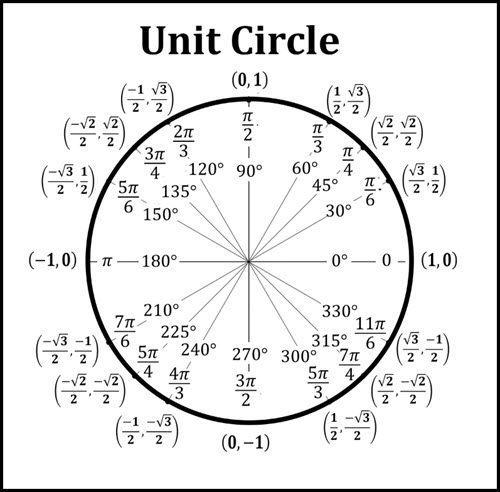
\includegraphics{unitcircle.jpg}	
\end{document}